\documentclass[10pt,a4paper]{report}
\usepackage[utf8]{inputenc}
\usepackage[english]{babel}
\usepackage{amsmath}
\usepackage{amsfonts}
\usepackage{amssymb}
\usepackage{graphicx}
\usepackage[left=2cm,right=2cm,top=2cm,bottom=2cm]{geometry}
\usepackage[autostyle, italian=quotes]{csquotes}
\author{Daniele Gilio}
\title{Exam Assignment}
\begin{document}
\section{Introduction}
This assignment was about text classification. We had to classify News titles by their topic; our classes were \enquote{science}, \enquote{health}, \enquote{business} and \enquote{entertainment}. Our raw features were the title itself and the publisher. The dataset was already divided in $10000$ training samples, $1000$ validation samples and $1000$ test samples. Our objective is to create a feature extraction process and to build one or more classifiers.
\section{Feature Extraction}
Since we are dealing with text classification we chose to employ the Bag of Words representation to encode the titles. In order to do that we had to build a fixed size dictionary. In Figure \ref{fig:acc_vs_dic} we can see how the dictionary size affects the performance of the models we intend to build.
\begin{figure}[!ht]
\centering
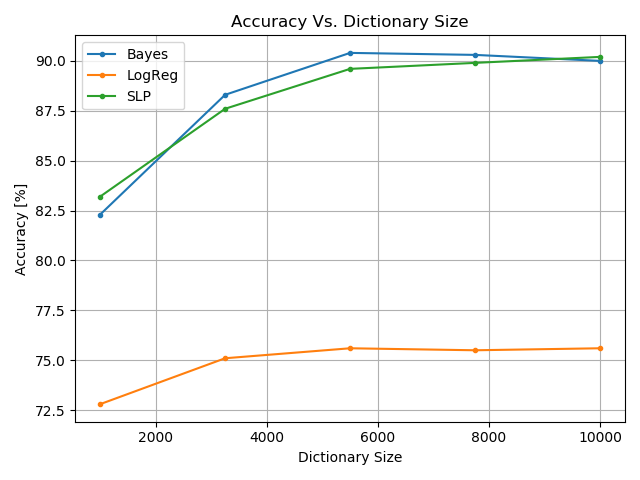
\includegraphics[width=0.5\linewidth]{acc_vs_dic.png}
\caption{Test Accuracy vs. Dictionary Size}
\label{fig:acc_vs_dic}
\end{figure}
Our goal with Figure \ref{fig:acc_vs_dic} was not to find the optimal dictionary size but to see if a bigger dictionary implied a better performance and this seems to be the case. Another decision we had to make was choosing if the publisher was a useful feature to keep. As we can see from Figure (), the $19$ different publishers mostly belong to a couple of classes. Based on that information we decide to keep the publisher information and we concatenated it to the title BoW. The simplest solution we found to encode the publishers was just to number them from $0$ to $18$. We also took into consideration normalization techniques, both in terms of words normalization (remove common words from the dictionary and stemming) and BoW normalization. We found out that using only one word normalization technique worsened the performance of all the models but using them both made them perform better. That said we used word normalization techniques for all the test we performed. Each model reacted differently to different BoW normalizations so we will discuss them separately.  
\section{Classifiers}
We decided to build a total of $4$ classifiers: Multinomial Bayesian Classifier, Multinomial Logistic Regression, Single Layer Perceptron and Multi-Layer Perceptron. The first two choices were biased upon the results we obtained in the Sentiment Analysis assignment. The latter two were chosen because of their versatility and previous assignments results.  
\subsection{Multinomial Naive Bayesian Classifier}
\subsection{Multinomial Logistic Regression}
\subsection{Single Layer Perceptron}
\subsection{Multi-Layer Perceptron}
\section{Results Analysis}
\section{Conclusions}
\end{document}